%!TEX program = xelatex
%%%%%%%%%%%%%%%%%%%%%%%这是导言部分的开始%%%%%%%%

%========= 导言部分声明文档的类型=================
\documentclass{article}

%=========导言部分可可以加载宏包=================
\usepackage{amsmath}                % 数学公式排版宏包
\usepackage{amssymb}                % 数学符号命令宏包
\usepackage{amsthm}                 % 数学定理宏包
\usepackage[UTF8]{ctex}             % 中文输入宏包
\usepackage[a4paper]{geometry}      % 页面设置宏包
\usepackage{setspace}               % 行间距宏包
\usepackage{graphicx}               % 图片宏包
\usepackage{listings}               % 代码宏包
\usepackage{color}					% 颜色宏包
\usepackage{xcolor}                 % 颜色处理宏包
\usepackage{float}                  % 浮动对象式样宏包
\usepackage{fontspec}
\usepackage{enumerate}				% 列举编号包

%=========页面设置==============================
\geometry{left=1cm,right=1cm,top=1cm,bottom=2cm}
\onehalfspacing
\setlength\parindent{0em}

%=========代码格式设置============================
\definecolor{dkgreen}{rgb}{0,0.6,0}
\definecolor{gray}{rgb}{0.5,0.5,0.5}
\definecolor{mauve}{rgb}{0.58,0,0.82}
% \setmonofont{Consolas}
\lstset{
	numbers = left, 	
	numberstyle = \color{gray}, 
	keywordstyle = \color{blue},
	commentstyle = \color{dkgreen}, 
	stringstyle = \color{mauve},
	basicstyle = \ttfamily,
	breaklines = true,
	frame = shadowbox, % 阴影效果
	rulesepcolor = \color{ red!20!green!20!blue!20} ,
	escapeinside = ``, % 英文分号中可写入中文
	xleftmargin = 2em,xrightmargin=2em, aboveskip=1em,
	framexleftmargin = 2em
} 

%=========导言部分可以定义标题信息===============
\title{组会报告}
\author{徐益}
\date{\today}
%%%%%%%%%%%%%%%%%%%%%%%这是导言部分的结束%%%%%%%%%

%%%%%%%%%%%%%%%%%%%%%%%这是正文部分的开始%%%%%%%%%
\begin{document}

%=========生成标题================================
\maketitle

%=========开始正文的输入==========================

%===========第一节=================
\section{工作内容} 
1. 完善原5GNR单线程测试程序;

2. 设计基于子载波分割的系统结果。

3. 实现基于子载波分割的单线程系统。

%===========第二节=================
\section{完善原5GNR单线程测试程序}
\begin{lstlisting}
# test_tb_sgl_thrd

vesion 1.2

Build and Execution Instructions
==============================

### Build:
> make

### Execution:
> ./main [-f filename]

### Clean:
> make clean

Change Log for Releases
==============================
## version 1.2
    * 支持文件读取配置信息
    * 选择mkl的随机数生产函数
    * 使用fread代替原先的channel信息读取函数

## version 1.1
    * 修复了基于Base Graph 2的编码器异常问题
    * 选择更灵活的导频初始化方案
    * 实现有效子载波数的变化    

## version 1.0
    * 实现了基于AVX2的5G LDPC编码器
    * 实现了基于AVX2的High-Throughput OMS及NMS译码器
    * 实现了基于AVX2的Low-Latency OMS及NMS译码器
    * 搭建了AWGN信道的5G LDPC编译码性能测试平台
\end{lstlisting}

%===========第三节=================
\section{基于子载波分割的系统结果}
\begin{figure}[H]
	\centering
	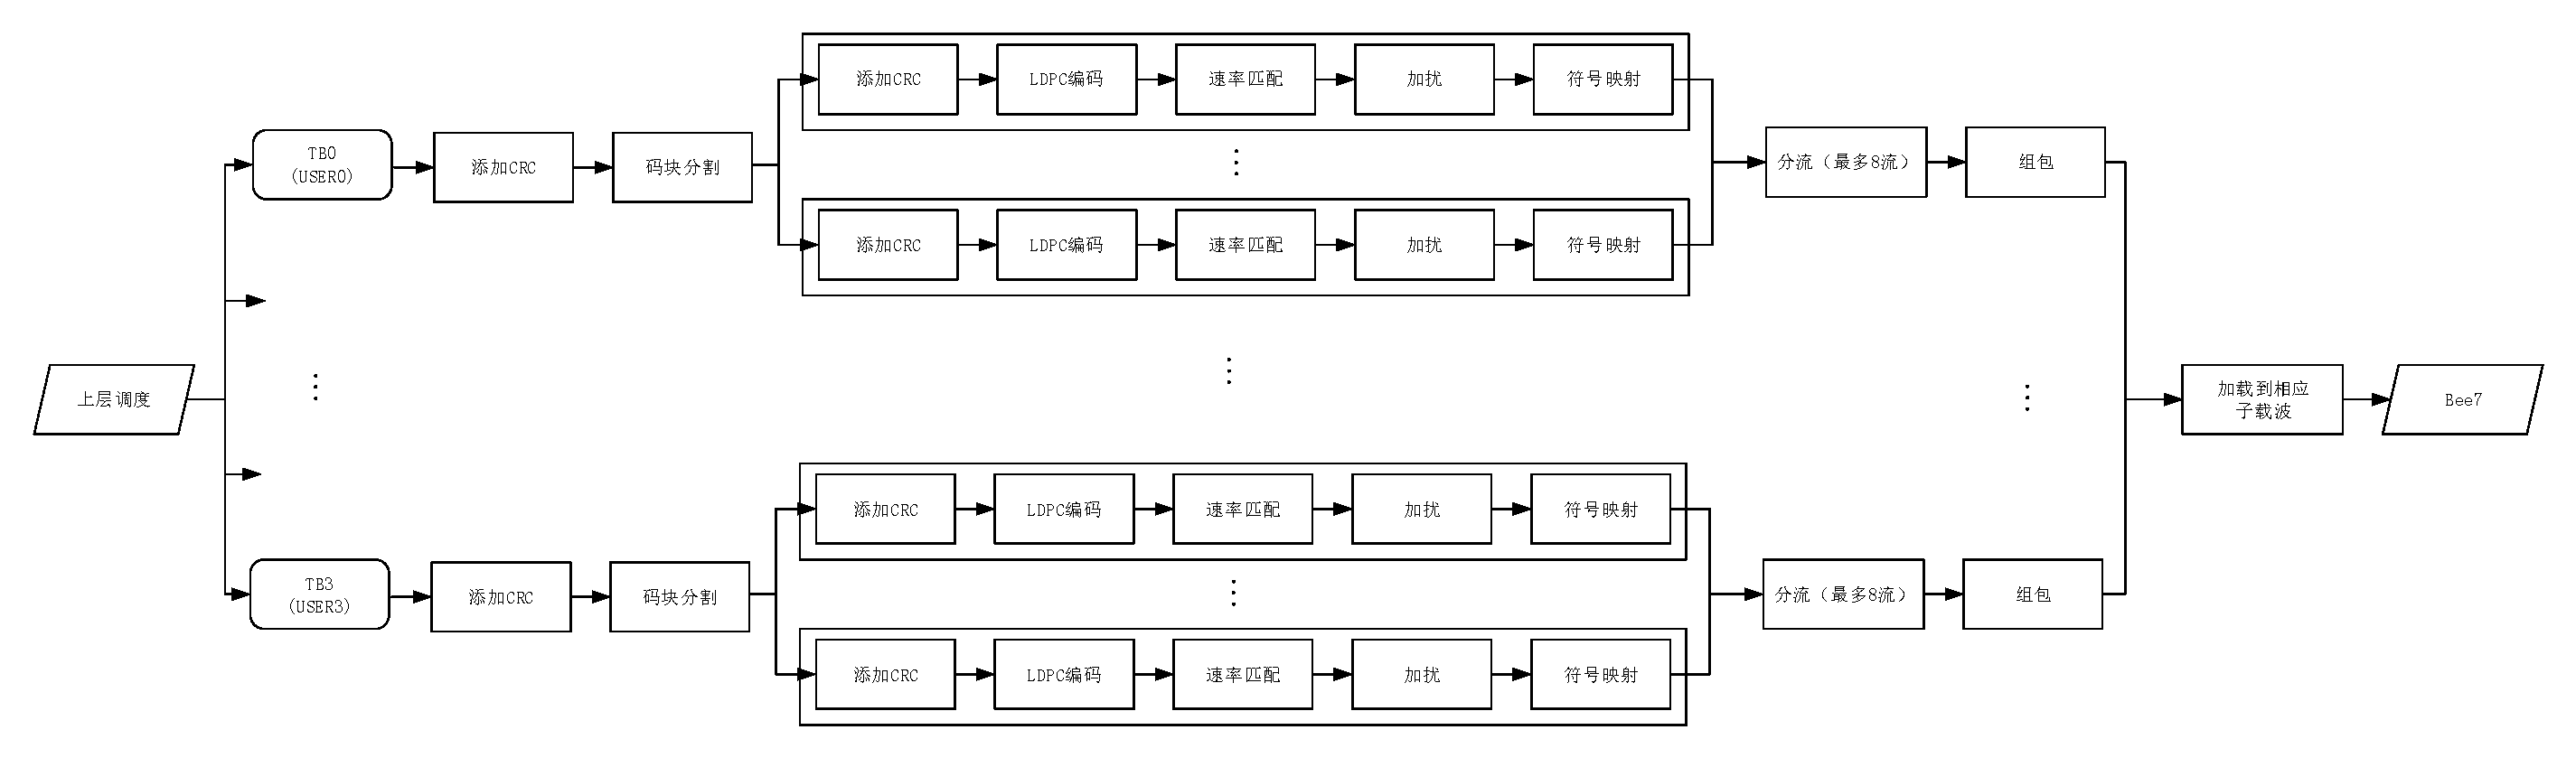
\includegraphics[width = \textwidth]{txstru.pdf}
	\caption{Tx端系统结构}
\end{figure}
\begin{figure}[H]
	\centering
	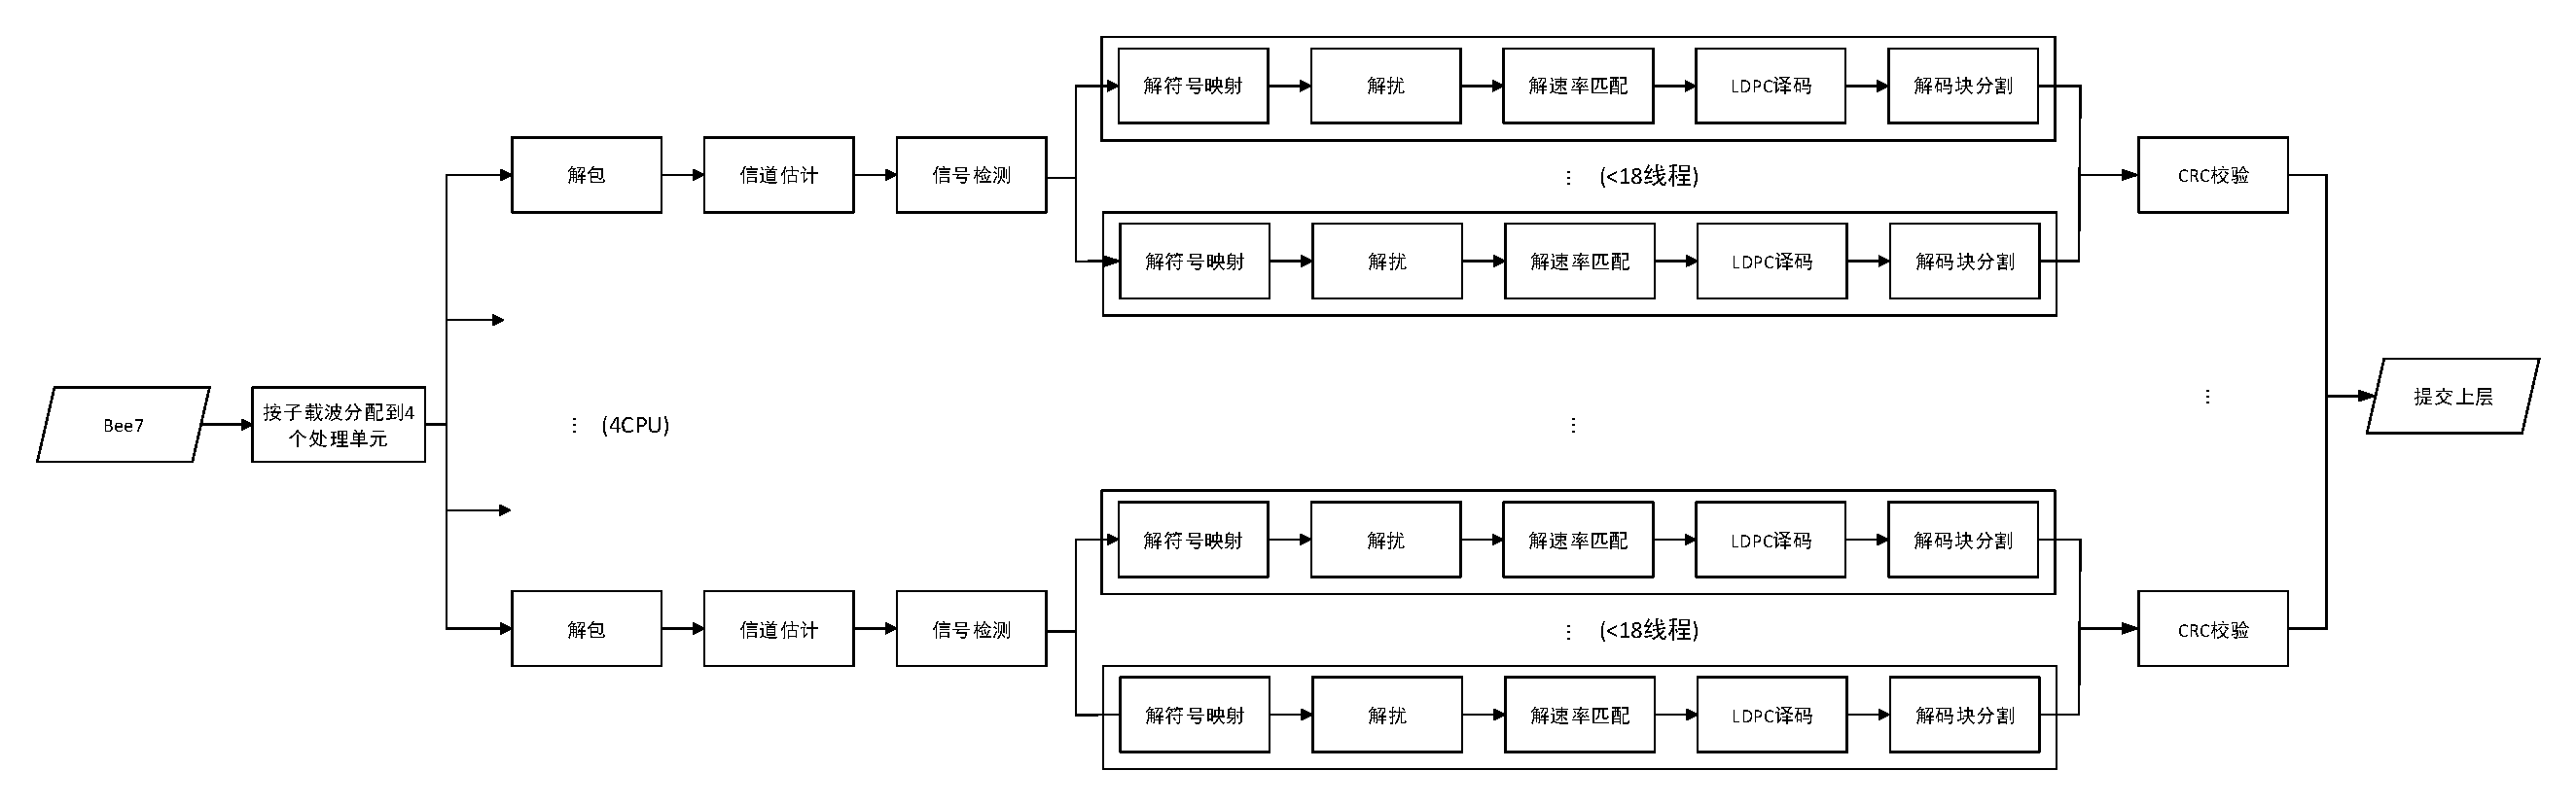
\includegraphics[width = \textwidth]{rxstru.pdf}
	\caption{Rx端系统结构}
\end{figure}

%===========第四节=================
\section{测试结果}
\begin{lstlisting}
==================== Test No. 1 ====================
SNR:      30.00
Subframe: 1000
---------------------- USER 0 ----------------------
CQI:    28(Q = 6, R = 948)
Stream: 1
-------------------- Throughput --------------------
tx_time:         0.2110s
rx_time:         0.5880s
tx_throughput:  86.7473Mbps
rx_throughput:  31.1282Mbps
-------------------- Error Rate --------------------
BER:    0.00e+00(0/18304000)
FER:    0.00e+00(0/1000)
----------------------------------------------------
---------------------- USER 1 ----------------------
CQI:    27(Q = 6, R = 910)
Stream: 1
-------------------- Throughput --------------------
tx_time:         0.2019s
rx_time:         0.5822s
tx_throughput:  87.0252Mbps
rx_throughput:  30.1751Mbps
-------------------- Error Rate --------------------
BER:    0.00e+00(0/17568000)
FER:    0.00e+00(0/1000)
----------------------------------------------------
---------------------- USER 2 ----------------------
CQI:    26(Q = 6, R = 873)
Stream: 1
-------------------- Throughput --------------------
tx_time:         0.1999s
rx_time:         0.5902s
tx_throughput:  84.3236Mbps
rx_throughput:  28.5615Mbps
-------------------- Error Rate --------------------
BER:    0.00e+00(0/16856000)
FER:    0.00e+00(0/1000)
----------------------------------------------------
---------------------- USER 3 ----------------------
CQI:    25(Q = 6, R = 822)
Stream: 1
-------------------- Throughput --------------------
tx_time:         0.2020s
rx_time:         0.6006s
tx_throughput:  78.5387Mbps
rx_throughput:  26.4139Mbps
-------------------- Error Rate --------------------
BER:    0.00e+00(0/15864000)
FER:    0.00e+00(0/1000)
----------------------------------------------------
====================================================

==================== Test No. 2 ====================
SNR:      30.00
Subframe: 1000
---------------------- USER 0 ----------------------
CQI:    28(Q = 6, R = 948)
Stream: 8
-------------------- Throughput --------------------
tx_time:         1.1928s
rx_time:         6.1965s
tx_throughput: 122.9147Mbps
rx_throughput:  23.6609Mbps
-------------------- Error Rate --------------------
BER:    8.38e-02(12284381/146616000)
FER:    1.00e+00(1000/1000)
----------------------------------------------------
---------------------- USER 1 ----------------------
CQI:    27(Q = 6, R = 910)
Stream: 7
-------------------- Throughput --------------------
tx_time:         0.9922s
rx_time:         5.2682s
tx_throughput: 124.1132Mbps
rx_throughput:  23.3748Mbps
-------------------- Error Rate --------------------
BER:    0.00e+00(0/123144000)
FER:    0.00e+00(0/1000)
----------------------------------------------------
---------------------- USER 2 ----------------------
CQI:    26(Q = 6, R = 873)
Stream: 6
-------------------- Throughput --------------------
tx_time:         0.8729s
rx_time:         4.5764s
tx_throughput: 115.9995Mbps
rx_throughput:  22.1259Mbps
-------------------- Error Rate --------------------
BER:    0.00e+00(0/101256000)
FER:    0.00e+00(0/1000)
----------------------------------------------------
---------------------- USER 3 ----------------------
CQI:    25(Q = 6, R = 822)
Stream: 5
-------------------- Throughput --------------------
tx_time:         0.7178s
rx_time:         3.8162s
tx_throughput: 110.6650Mbps
rx_throughput:  20.8166Mbps
-------------------- Error Rate --------------------
BER:    0.00e+00(0/79440000)
FER:    0.00e+00(0/1000)
----------------------------------------------------
====================================================
\end{lstlisting}

%===========第五节=================
\section{有PRACH情况下的资源分配问题}
\begin{figure}[H]
	\centering
	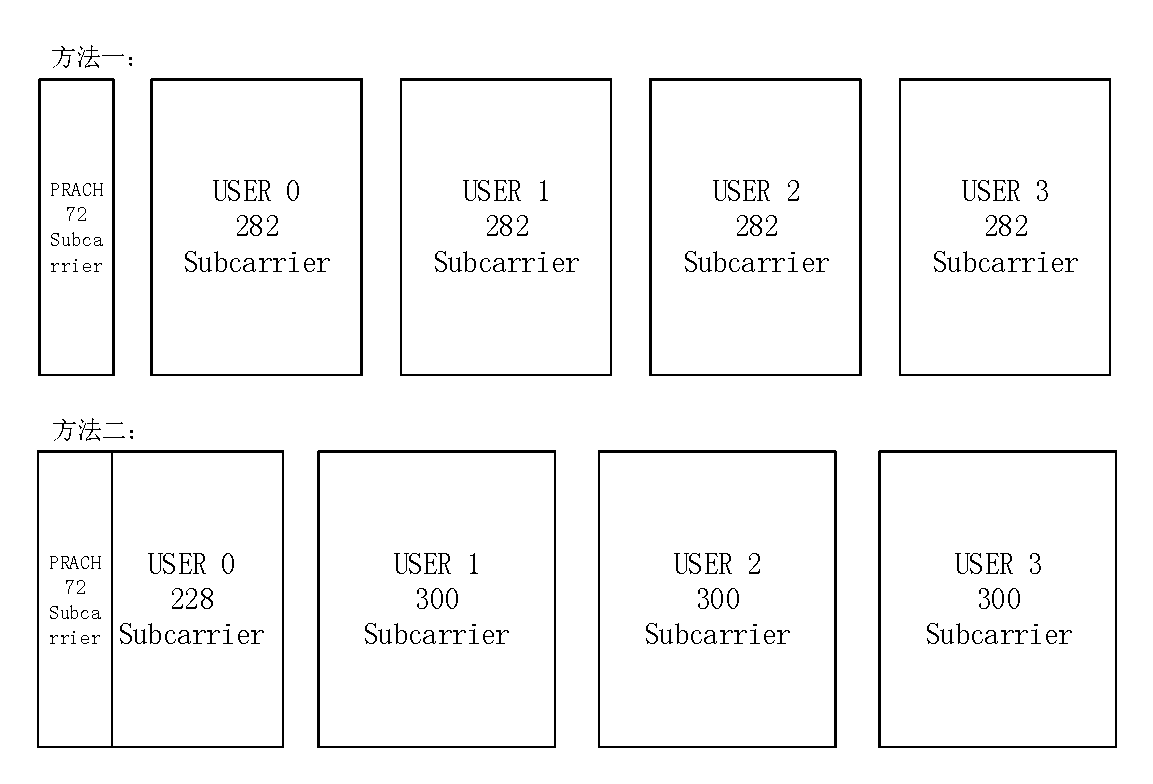
\includegraphics[width = \textwidth]{ques.pdf}
	\caption{两种方案}
\end{figure}

%===========下周计划=================
% \section{下阶段计划}
% 1. 完善单线程系统(修复Bug)

\end{document}
%%%%%%%%%%%%%%%%%%%%%%%这是正文部分的结束%%%%%%%%%%%%